\documentclass{standalone}
\usepackage{tikz}
\usepackage{amsmath}

\usetikzlibrary{automata,positioning}
 
\usetikzlibrary{positioning}
\begin{document}
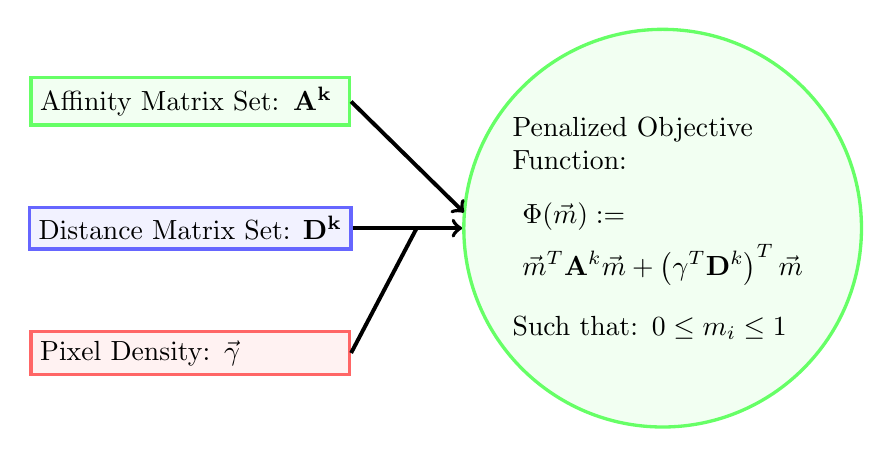
\begin{tikzpicture}[
roundnode/.style={circle, draw=green!60, fill=green!5, very thick, minimum size=7mm},
rsquarenode/.style={rectangle, draw=red!60, fill=red!5, very thick, minimum size=5mm},
bsquarenode/.style={rectangle, draw=blue!60, fill=blue!5, very thick, minimum size=5mm},
gsquarenode/.style={rectangle, draw=green!60, fill=green!5, very thick, minimum size=5mm},
]
%Nodes
\node[bsquarenode](a0) at (0,0){Distance Matrix Set: $\mathbf{D^k}$};


\node[gsquarenode](d0)[above=of a0,text width=1.5in]{Affinity Matrix Set: $\mathbf{A^k}$};


\node[rsquarenode](g0)[below=of a0,text width=1.5in]{Pixel Density: $\vec{\gamma}$};

% \node(none) at (6,-1.5) {adsf};

\node[roundnode](d1) at (6,0)[text width=1.5in]{Penalized Objective Function:
\[
\begin{split}
&\Phi(\vec{m}) : =\\ &\vec{m}^T\mathbf{A}^k\vec{m}+\left(\gamma^T\mathbf{D}^k\right)^T\vec{m} 
\end{split}
\]
Such that: $0\le m_i \le 1$
};

\node(none) at (3,0){};


\draw[line width=0.5mm,->] (a0.east) -- (d1.west);

\draw[line width=0.5mm,-] (g0.east) -- (none.west);

\node(none) at (3.6,0.2){};
 
\draw[line width=0.5mm,->] (d0.east) -- (none.west);


% \node[bsquarenode](gamma)[above=of out,text width=1in] {\centering Pixel Density:\\\vspace{.1in}$\vec{\gamma}: =
%     \begin{bmatrix}
%         \gamma_0\\\gamma_1\\\gamma_2\\\vdots\\\gamma_n
%     \end{bmatrix}$ };

% \node[rsquarenode](sim)[below=of out,text width=2.5in] {\centering Similarity Matrix:\\\vspace{.1in}$\mathbf{\tilde{S}}: =
%     \begin{bmatrix}
%         s_{0,0}&  s_{0,1}&  s_{0,2}& {}& \dots& {}& s_{0, n}\\
%         s_{1,0}&  s_{1,1}&  s_{1,2}& {}& \dots& {}& s_{1, n}\\
%         s_{2,0}&  s_{2,1}&  s_{2,2}& {}& \dots& {}& s_{2, n}\\
%         {}&{}&{}&{}&{}&{}\\
%         \vdots& \vdots&  \vdots& {}&\ddots & {}&{}\\
%         {}&{}&{}&{}&{}&{}\\
%         s_{n,0}&  s_{n,1}&  s_{n,2}& {}& \dots& {}& s_{n, n}\\
%     \end{bmatrix}$};

% \node[bsquarenode](gamma_m)[right=of gamma,text width=2in] {\centering Vertex Weights:\\\vspace{.1in}$\mathbf{\Gamma}: =
%     \begin{bmatrix}
%         \gamma_{0}&{}&{}&{}&{}\\
%         {}&\gamma_{1}&{}&{}&{}&\\
%         {}&{}&\gamma_{2}&{}&{}&\\
%         {}&{}&{}&\ddots&{}&\\
%         {}&{}&{}&{}&\gamma_{n}\\
%     \end{bmatrix}$ };

% \node(none) at (6,0) {};

% \node[gsquarenode](aff)[right=of none,text width=3in] {\centering Affinity Matrix:\\\vspace{.1in}$\mathbf{A}: = \mathbf{\Gamma \tilde{S} \Gamma} = 
%     \begin{bmatrix}
%         a_{0,0}&  a_{0,1}&  a_{0,2}& {}& \dots& {}& a_{0, n}\\
%         a_{1,0}&  a_{1,1}&  a_{1,2}& {}& \dots& {}& a_{1, n}\\
%         a_{2,0}&  a_{2,1}&  a_{2,2}& {}& \dots& {}& a_{2, n}\\
%         {}&{}&{}&{}&{}&{}\\
%         \vdots& \vdots&  \vdots& {}&\ddots & {}&{}\\
%         {}&{}&{}&{}&{}&{}\\
%         a_{n,0}&  a_{n,1}&  a_{n,2}& {}& \dots& {}& a_{n, n}\\
%     \end{bmatrix}$ };

%Lines
% \draw[line width=0.5mm,->] (data.east) -- (out.west);
% \draw[line width=0.5mm,<-] (gamma.south) -- (out.north);
% \draw[line width=0.5mm,->] (gamma.east) -- (gamma_m.west);
% \draw[line width=0.5mm,<-] (sim.north) -- (out.south);
% \draw[line width=0.5mm,->] (sim.east) -- (aff.south);
% \draw[line width=0.5mm,->] (gamma_m.south) -- (aff.north);









\end{tikzpicture}
\end{document}
